\documentclass{article}
\usepackage[utf8]{inputenc}
\usepackage{tikz}
\usepackage{float}

\tikzstyle{input} = [draw,trapezium,trapezium left angle=120,trapezium right angle=60]
\tikzstyle{output} = [draw,trapezium,trapezium left angle=60,trapezium right angle=120]
\tikzstyle{block} = [draw, rectangle, minimum height=2.5em, minimum width=5em]

\title{ICSI412 Project 1: Documentation}
\author{Huang Kaisheng <2020215138@stu.cqupt.edu.cn>}
\date{Apr. 30th, 2023}

\begin{document}

\maketitle
\newpage

\tableofcontents
\newpage


\section{System Documentation}
This section contains a high-level data flow diagram, list of routines and brief descriptions and some implementation details.
\subsection{High-level Data Flow Diagram}
Figure 1 shows the high level data flow diagram.
\begin{figure}[H]
\begin{tikzpicture}[->,>=stealth',node distance=2cm,auto]
    \node[input] (in) {Standard Input / Redirected Input File};
    \node[block, below of=in] (A) {Program A};
    \node[block, right of=A] (B) {Program B};
    \node[block, right of=B] (C) {Program C};
    \node[output, below of=C] (out) {Standard Output / Redirected Output File};
    
    \draw[->] (in) -- (A);
    \draw[->] (A) -- (B);
    \draw[->] (B) -- (C);
    \draw[->] (C) -- (out);
\end{tikzpicture}
\caption{Data Flow Diagram}
\end{figure}

\subsection{List of Routines and Brief Descriptions}
\begin{table}[h]
\centering
\begin{tabular}{|p{4cm}|p{9cm}|}
\hline
\textbf{Function} & \textbf{Description} \\ \hline
\texttt{execute\_command} & Forks and executes the commands specified in the \texttt{command} array. The \texttt{input\_fd} parameter specifies the file descriptor to replace the standard input, and \texttt{output\_fd} specifies the file descriptor to replace standard output. Returns -1 if an error occurs, and 0 otherwise. \\ \hline
\texttt{execute\_piped\_command} & Creates a pipeline between commands specified in the \texttt{commands} array and executes them. Uses the file descriptor array specified in the \texttt{pipes} parameter for communication between commands. The \texttt{file\_remap} parameter specifies the stdin and stdout redirection map. Returns -1 if an error occurs, and 0 otherwise. \\ \hline
\texttt{parse\_command} & Parses the command string specified in the \texttt{command} parameter, and stores the results in the \texttt{commands} parameter. The stdin and stdout redirection map is stored in the \texttt{file\_remap} parameter, and the number of commands parsed is stored in the \texttt{num\_commands} parameter. Returns -1 if an error occurs, and 0 otherwise. \\ \hline
\end{tabular}
\end{table}

\subsection{Implementation Details}
The program shown above is a shell program that allows the user to input commands and execute them.

The \texttt{execute.c} file contains two functions: \\
1. \texttt{execute\_command()} takes a command array, input file descriptor and output file descriptor as arguments. It forks a new process to run the command and redirects stdin and stdout to the input and output file descriptors, respectively. It returns 0 if successful and -1 if there was an error.  \\
2. \texttt{execute\_piped\_command()} takes a 2D array of commands, an array of file descriptors for pipes, an array of file names for input and output redirection, and the number of commands as arguments. It creates multiple pipes and forks a new process for each command. It redirects input and output either to the appropriate pipe or the specified input/output file. It returns 0 if successful and -1 if there was an error. 

The \texttt{mysh.c} file is the main program that reads user input, parses the commands, and executes them. It uses \texttt{fgets()} to read input from the user, and passes the input to \texttt{parse\_command()} and \texttt{execute\_piped\_command()} to parse and execute the commands, respectively.

The \texttt{parser.c} file contains the \texttt{parse\_command()} function, which takes a command string, an array of command arrays, an array of filenames for input/output redirection, and an int pointer to the number of commands. It splits the command string into tokens and saves each token to the appropriate command array. It also handles input/output redirection and single quotes in the command string. It returns 0 if successful and 1 if there was an error.

\section{Test Documentation}
This section contains the description of test method, and a test result.
\subsection{Test Method}
I wrote a naive shell script to make the test, whose procedure is: \\
1. Read the test suite definition and make two temporary directories, one for our shell and another one for the system shell, to compare the result. \\
2. Run \texttt{make} to build the program. \\
3. Run our shell with the shell script in test suite, and run the system shell with the shell script in test suite. \\
4. Run \texttt{diff} to compare the results and check if the output is same.

\subsection{Test Result}
With the test suite provided in the homework document:
\begin{verbatim}
victor@victor-dev:~/CSI412/Project1(master○) » make test 
./test/test.sh countryCity
make[1]: Entering directory '/home/victor/CSI412/Project1'
gcc -c -o mysh.o mysh.c -I.
gcc -c -o execute.o execute.c -I.
gcc -c -o parser.o parser.c -I.
gcc -o mysh mysh.o execute.o parser.o -I.
make[1]: Leaving directory '/home/victor/CSI412/Project1'
Using test suite countryCity:
cat country.txt city.txt  | egrep 'g' | sort | more > countryCitygSorted.txt
cat country.txt city.txt  | egrep 'g' | sort | wc -l > countryCitygCount.txt
Testing program: 

Making system shell sample: 
+ cat country.txt city.txt
+ egrep g
+ sort
+ more
+ cat country.txt city.txt
+ egrep g
+ wc -l
+ sort
Making diff...
✅ countryCitygSorted.txt       TEST PASSED!
✅ countryCitygCount.txt        TEST PASSED!
Removing artifacts...
\end{verbatim}

Running screenshot:

\begin{figure}[H]
    \centering
    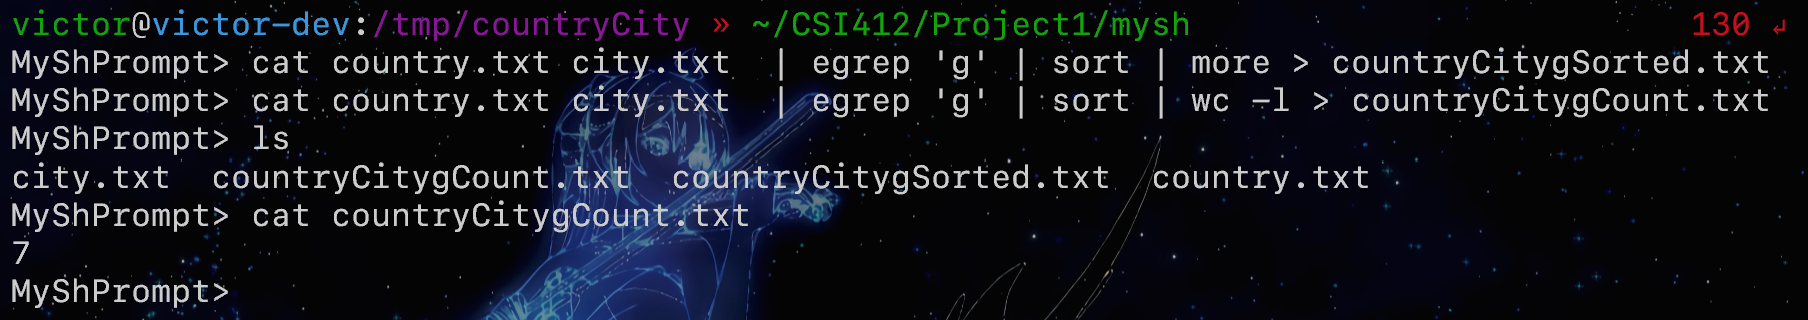
\includegraphics[width=15cm, screenshot]{img/project1_run_result.png}
    \caption{The screenshot of shell}
\end{figure}

\section{User Documentation}
This section contains how to build the program and argument definition.

\subsection{How to run the program}
Make sure that there is a C compiler and GNU make in your environment. \\
Run \texttt{make} to compile the program. \\
And the binary will appear at \texttt{mysh}.

\subsection{Argument Definition}
The program receives 1 optional argument, which is the script to be interpreted.
\end{document}
